% Options for packages loaded elsewhere
\PassOptionsToPackage{unicode}{hyperref}
\PassOptionsToPackage{hyphens}{url}
%
\documentclass[
]{article}
\usepackage{amsmath,amssymb}
\usepackage{lmodern}
\usepackage{iftex}
\ifPDFTeX
  \usepackage[T1]{fontenc}
  \usepackage[utf8]{inputenc}
  \usepackage{textcomp} % provide euro and other symbols
\else % if luatex or xetex
  \usepackage{unicode-math}
  \defaultfontfeatures{Scale=MatchLowercase}
  \defaultfontfeatures[\rmfamily]{Ligatures=TeX,Scale=1}
\fi
% Use upquote if available, for straight quotes in verbatim environments
\IfFileExists{upquote.sty}{\usepackage{upquote}}{}
\IfFileExists{microtype.sty}{% use microtype if available
  \usepackage[]{microtype}
  \UseMicrotypeSet[protrusion]{basicmath} % disable protrusion for tt fonts
}{}
\makeatletter
\@ifundefined{KOMAClassName}{% if non-KOMA class
  \IfFileExists{parskip.sty}{%
    \usepackage{parskip}
  }{% else
    \setlength{\parindent}{0pt}
    \setlength{\parskip}{6pt plus 2pt minus 1pt}}
}{% if KOMA class
  \KOMAoptions{parskip=half}}
\makeatother
\usepackage{xcolor}
\IfFileExists{xurl.sty}{\usepackage{xurl}}{} % add URL line breaks if available
\IfFileExists{bookmark.sty}{\usepackage{bookmark}}{\usepackage{hyperref}}
\hypersetup{
  hidelinks,
  pdfcreator={LaTeX via pandoc}}
\urlstyle{same} % disable monospaced font for URLs
\usepackage[margin=1in]{geometry}
\usepackage{color}
\usepackage{fancyvrb}
\newcommand{\VerbBar}{|}
\newcommand{\VERB}{\Verb[commandchars=\\\{\}]}
\DefineVerbatimEnvironment{Highlighting}{Verbatim}{commandchars=\\\{\}}
% Add ',fontsize=\small' for more characters per line
\usepackage{framed}
\definecolor{shadecolor}{RGB}{248,248,248}
\newenvironment{Shaded}{\begin{snugshade}}{\end{snugshade}}
\newcommand{\AlertTok}[1]{\textcolor[rgb]{0.94,0.16,0.16}{#1}}
\newcommand{\AnnotationTok}[1]{\textcolor[rgb]{0.56,0.35,0.01}{\textbf{\textit{#1}}}}
\newcommand{\AttributeTok}[1]{\textcolor[rgb]{0.77,0.63,0.00}{#1}}
\newcommand{\BaseNTok}[1]{\textcolor[rgb]{0.00,0.00,0.81}{#1}}
\newcommand{\BuiltInTok}[1]{#1}
\newcommand{\CharTok}[1]{\textcolor[rgb]{0.31,0.60,0.02}{#1}}
\newcommand{\CommentTok}[1]{\textcolor[rgb]{0.56,0.35,0.01}{\textit{#1}}}
\newcommand{\CommentVarTok}[1]{\textcolor[rgb]{0.56,0.35,0.01}{\textbf{\textit{#1}}}}
\newcommand{\ConstantTok}[1]{\textcolor[rgb]{0.00,0.00,0.00}{#1}}
\newcommand{\ControlFlowTok}[1]{\textcolor[rgb]{0.13,0.29,0.53}{\textbf{#1}}}
\newcommand{\DataTypeTok}[1]{\textcolor[rgb]{0.13,0.29,0.53}{#1}}
\newcommand{\DecValTok}[1]{\textcolor[rgb]{0.00,0.00,0.81}{#1}}
\newcommand{\DocumentationTok}[1]{\textcolor[rgb]{0.56,0.35,0.01}{\textbf{\textit{#1}}}}
\newcommand{\ErrorTok}[1]{\textcolor[rgb]{0.64,0.00,0.00}{\textbf{#1}}}
\newcommand{\ExtensionTok}[1]{#1}
\newcommand{\FloatTok}[1]{\textcolor[rgb]{0.00,0.00,0.81}{#1}}
\newcommand{\FunctionTok}[1]{\textcolor[rgb]{0.00,0.00,0.00}{#1}}
\newcommand{\ImportTok}[1]{#1}
\newcommand{\InformationTok}[1]{\textcolor[rgb]{0.56,0.35,0.01}{\textbf{\textit{#1}}}}
\newcommand{\KeywordTok}[1]{\textcolor[rgb]{0.13,0.29,0.53}{\textbf{#1}}}
\newcommand{\NormalTok}[1]{#1}
\newcommand{\OperatorTok}[1]{\textcolor[rgb]{0.81,0.36,0.00}{\textbf{#1}}}
\newcommand{\OtherTok}[1]{\textcolor[rgb]{0.56,0.35,0.01}{#1}}
\newcommand{\PreprocessorTok}[1]{\textcolor[rgb]{0.56,0.35,0.01}{\textit{#1}}}
\newcommand{\RegionMarkerTok}[1]{#1}
\newcommand{\SpecialCharTok}[1]{\textcolor[rgb]{0.00,0.00,0.00}{#1}}
\newcommand{\SpecialStringTok}[1]{\textcolor[rgb]{0.31,0.60,0.02}{#1}}
\newcommand{\StringTok}[1]{\textcolor[rgb]{0.31,0.60,0.02}{#1}}
\newcommand{\VariableTok}[1]{\textcolor[rgb]{0.00,0.00,0.00}{#1}}
\newcommand{\VerbatimStringTok}[1]{\textcolor[rgb]{0.31,0.60,0.02}{#1}}
\newcommand{\WarningTok}[1]{\textcolor[rgb]{0.56,0.35,0.01}{\textbf{\textit{#1}}}}
\usepackage{graphicx}
\makeatletter
\def\maxwidth{\ifdim\Gin@nat@width>\linewidth\linewidth\else\Gin@nat@width\fi}
\def\maxheight{\ifdim\Gin@nat@height>\textheight\textheight\else\Gin@nat@height\fi}
\makeatother
% Scale images if necessary, so that they will not overflow the page
% margins by default, and it is still possible to overwrite the defaults
% using explicit options in \includegraphics[width, height, ...]{}
\setkeys{Gin}{width=\maxwidth,height=\maxheight,keepaspectratio}
% Set default figure placement to htbp
\makeatletter
\def\fps@figure{htbp}
\makeatother
\setlength{\emergencystretch}{3em} % prevent overfull lines
\providecommand{\tightlist}{%
  \setlength{\itemsep}{0pt}\setlength{\parskip}{0pt}}
\setcounter{secnumdepth}{-\maxdimen} % remove section numbering
\ifLuaTeX
  \usepackage{selnolig}  % disable illegal ligatures
\fi

\author{}
\date{\vspace{-2.5em}}

\begin{document}

Investigación reproducible: Tareas calificadas por los compañeros Course
Project 1

Cargar los datos

\begin{Shaded}
\begin{Highlighting}[]
\NormalTok{activity\_data }\OtherTok{\textless{}{-}} \FunctionTok{read.csv}\NormalTok{(}\StringTok{"./data/activity.csv"}\NormalTok{)}
\end{Highlighting}
\end{Shaded}

preprocesar los datos

\begin{Shaded}
\begin{Highlighting}[]
\FunctionTok{names}\NormalTok{(activity\_data)}
\end{Highlighting}
\end{Shaded}

\begin{verbatim}
## [1] "steps"    "date"     "interval"
\end{verbatim}

\begin{Shaded}
\begin{Highlighting}[]
\FunctionTok{head}\NormalTok{(activity\_data)}
\end{Highlighting}
\end{Shaded}

\begin{verbatim}
##   steps       date interval
## 1    NA 2012-10-01        0
## 2    NA 2012-10-01        5
## 3    NA 2012-10-01       10
## 4    NA 2012-10-01       15
## 5    NA 2012-10-01       20
## 6    NA 2012-10-01       25
\end{verbatim}

\begin{Shaded}
\begin{Highlighting}[]
\FunctionTok{summary}\NormalTok{(activity\_data)}
\end{Highlighting}
\end{Shaded}

\begin{verbatim}
##      steps            date              interval     
##  Min.   :  0.00   Length:17568       Min.   :   0.0  
##  1st Qu.:  0.00   Class :character   1st Qu.: 588.8  
##  Median :  0.00   Mode  :character   Median :1177.5  
##  Mean   : 37.38                      Mean   :1177.5  
##  3rd Qu.: 12.00                      3rd Qu.:1766.2  
##  Max.   :806.00                      Max.   :2355.0  
##  NA's   :2304
\end{verbatim}

¿Cuál es la media del número total de pasos dados por día?

\begin{enumerate}
\def\labelenumi{\arabic{enumi}.}
\tightlist
\item
  Calcular el número total de pasos dados por día
\end{enumerate}

\begin{Shaded}
\begin{Highlighting}[]
\NormalTok{steps\_day }\OtherTok{\textless{}{-}} \FunctionTok{aggregate}\NormalTok{(steps }\SpecialCharTok{\textasciitilde{}}\NormalTok{ date, activity\_data, sum, }\AttributeTok{na.rm=}\ConstantTok{TRUE}\NormalTok{)}
\NormalTok{steps\_day}
\end{Highlighting}
\end{Shaded}

\begin{verbatim}
##          date steps
## 1  2012-10-02   126
## 2  2012-10-03 11352
## 3  2012-10-04 12116
## 4  2012-10-05 13294
## 5  2012-10-06 15420
## 6  2012-10-07 11015
## 7  2012-10-09 12811
## 8  2012-10-10  9900
## 9  2012-10-11 10304
## 10 2012-10-12 17382
## 11 2012-10-13 12426
## 12 2012-10-14 15098
## 13 2012-10-15 10139
## 14 2012-10-16 15084
## 15 2012-10-17 13452
## 16 2012-10-18 10056
## 17 2012-10-19 11829
## 18 2012-10-20 10395
## 19 2012-10-21  8821
## 20 2012-10-22 13460
## 21 2012-10-23  8918
## 22 2012-10-24  8355
## 23 2012-10-25  2492
## 24 2012-10-26  6778
## 25 2012-10-27 10119
## 26 2012-10-28 11458
## 27 2012-10-29  5018
## 28 2012-10-30  9819
## 29 2012-10-31 15414
## 30 2012-11-02 10600
## 31 2012-11-03 10571
## 32 2012-11-05 10439
## 33 2012-11-06  8334
## 34 2012-11-07 12883
## 35 2012-11-08  3219
## 36 2012-11-11 12608
## 37 2012-11-12 10765
## 38 2012-11-13  7336
## 39 2012-11-15    41
## 40 2012-11-16  5441
## 41 2012-11-17 14339
## 42 2012-11-18 15110
## 43 2012-11-19  8841
## 44 2012-11-20  4472
## 45 2012-11-21 12787
## 46 2012-11-22 20427
## 47 2012-11-23 21194
## 48 2012-11-24 14478
## 49 2012-11-25 11834
## 50 2012-11-26 11162
## 51 2012-11-27 13646
## 52 2012-11-28 10183
## 53 2012-11-29  7047
\end{verbatim}

\begin{enumerate}
\def\labelenumi{\arabic{enumi}.}
\setcounter{enumi}{1}
\tightlist
\item
  histograma del número total de pasos dados cada día
\end{enumerate}

\begin{Shaded}
\begin{Highlighting}[]
\FunctionTok{hist}\NormalTok{(steps\_day}\SpecialCharTok{$}\NormalTok{steps, }\AttributeTok{main =} \StringTok{"Total number of steps taken per day"}\NormalTok{, }\AttributeTok{xlab =} \StringTok{"Total steps taken per day"}\NormalTok{, }\AttributeTok{col =} \StringTok{"darkblue"}\NormalTok{)}
\end{Highlighting}
\end{Shaded}

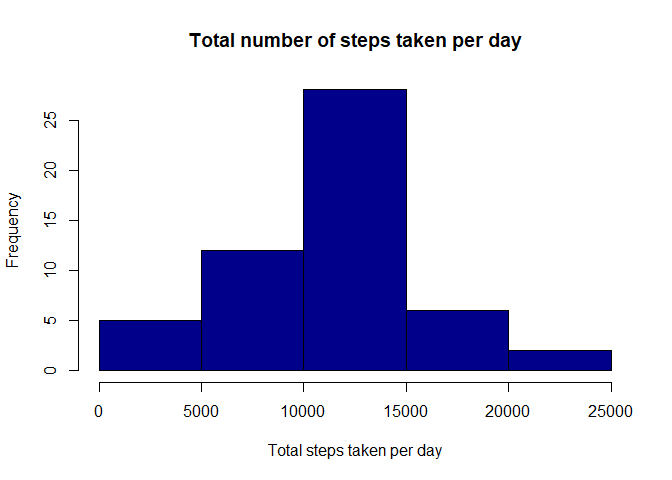
\includegraphics{reprodResearchProject1_files/figure-latex/unnamed-chunk-6-1.pdf}

\begin{enumerate}
\def\labelenumi{\arabic{enumi}.}
\setcounter{enumi}{2}
\tightlist
\item
  Calcule e informe la media y la mediana del número total de pasos
  dados por día
\end{enumerate}

\begin{Shaded}
\begin{Highlighting}[]
\NormalTok{mean\_steps\_day }\OtherTok{\textless{}{-}} \FunctionTok{mean}\NormalTok{(steps\_day}\SpecialCharTok{$}\NormalTok{steps)}
\NormalTok{mean\_steps\_day}
\end{Highlighting}
\end{Shaded}

\begin{verbatim}
## [1] 10766.19
\end{verbatim}

\begin{Shaded}
\begin{Highlighting}[]
\NormalTok{median\_steps\_day }\OtherTok{\textless{}{-}} \FunctionTok{median}\NormalTok{(steps\_day}\SpecialCharTok{$}\NormalTok{steps)}
\NormalTok{median\_steps\_day}
\end{Highlighting}
\end{Shaded}

\begin{verbatim}
## [1] 10765
\end{verbatim}

¿Cuál es el patrón de actividad diaria promedio?

\begin{enumerate}
\def\labelenumi{\arabic{enumi}.}
\tightlist
\item
  Gráfica de serie de tiempo del intervalo de 5 minutos
\end{enumerate}

\begin{Shaded}
\begin{Highlighting}[]
\NormalTok{steps\_interval}\OtherTok{\textless{}{-}}\FunctionTok{aggregate}\NormalTok{(steps}\SpecialCharTok{\textasciitilde{}}\NormalTok{interval, }\AttributeTok{data=}\NormalTok{activity\_data, mean, }\AttributeTok{na.rm=}\ConstantTok{TRUE}\NormalTok{)}
\FunctionTok{plot}\NormalTok{(steps}\SpecialCharTok{\textasciitilde{}}\NormalTok{interval, }\AttributeTok{data=}\NormalTok{steps\_interval, }\AttributeTok{type=}\StringTok{"l"}\NormalTok{, }\AttributeTok{col=}\StringTok{"darkblue"}\NormalTok{)}
\end{Highlighting}
\end{Shaded}

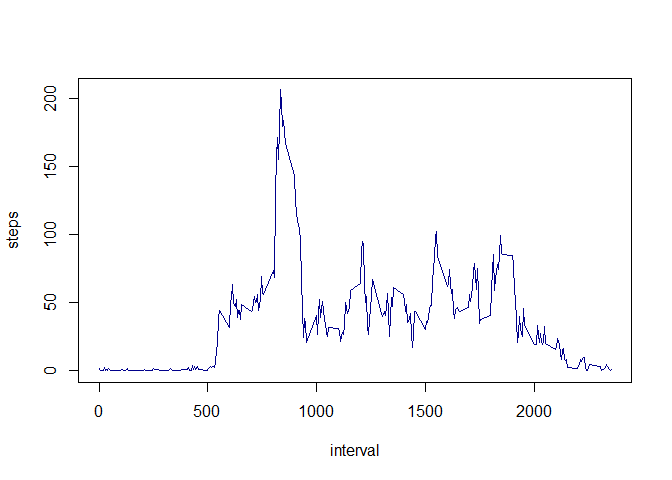
\includegraphics{reprodResearchProject1_files/figure-latex/unnamed-chunk-7-1.pdf}

\begin{enumerate}
\def\labelenumi{\arabic{enumi}.}
\setcounter{enumi}{1}
\tightlist
\item
  ¿Qué intervalo de 5 minutos, en promedio de todos los días del
  conjunto de datos, contiene la cantidad máxima de pasos?
\end{enumerate}

\begin{Shaded}
\begin{Highlighting}[]
\NormalTok{interval\_Max\_steps }\OtherTok{\textless{}{-}}\NormalTok{ steps\_interval[}\FunctionTok{which.max}\NormalTok{(steps\_interval}\SpecialCharTok{$}\NormalTok{steps),]}\SpecialCharTok{$}\NormalTok{interval}
\NormalTok{interval\_Max\_steps}
\end{Highlighting}
\end{Shaded}

\begin{verbatim}
## [1] 835
\end{verbatim}

Imputación de valores faltantes

\begin{enumerate}
\def\labelenumi{\arabic{enumi}.}
\tightlist
\item
  Número total de valores faltantes en el conjunto de datos
\end{enumerate}

\begin{Shaded}
\begin{Highlighting}[]
\NormalTok{values\_missings }\OtherTok{\textless{}{-}} \FunctionTok{sum}\NormalTok{(}\FunctionTok{is.na}\NormalTok{(activity\_data}\SpecialCharTok{$}\NormalTok{steps))}
\NormalTok{values\_missings}
\end{Highlighting}
\end{Shaded}

\begin{verbatim}
## [1] 2304
\end{verbatim}

\begin{enumerate}
\def\labelenumi{\arabic{enumi}.}
\setcounter{enumi}{1}
\tightlist
\item
  Estrategia para completar todos los valores que faltan en el conjunto
  de datos.
\end{enumerate}

\begin{Shaded}
\begin{Highlighting}[]
\NormalTok{mean\_steps\_interval}\OtherTok{\textless{}{-}}\ControlFlowTok{function}\NormalTok{(interval)\{}
\NormalTok{    steps\_interval[steps\_interval}\SpecialCharTok{$}\NormalTok{interval}\SpecialCharTok{==}\NormalTok{interval,]}\SpecialCharTok{$}\NormalTok{steps}
\NormalTok{\}}
\end{Highlighting}
\end{Shaded}

\begin{enumerate}
\def\labelenumi{\arabic{enumi}.}
\setcounter{enumi}{2}
\tightlist
\item
  Nuevo conjunto de datos igual al conjunto de datos original con los
  datos faltantes completados.
\end{enumerate}

\begin{Shaded}
\begin{Highlighting}[]
\NormalTok{activity\_data\_NA}\OtherTok{\textless{}{-}}\NormalTok{activity\_data}
\ControlFlowTok{for}\NormalTok{(i }\ControlFlowTok{in} \DecValTok{1}\SpecialCharTok{:}\FunctionTok{nrow}\NormalTok{(activity\_data\_NA))\{}
    \ControlFlowTok{if}\NormalTok{(}\FunctionTok{is.na}\NormalTok{(activity\_data\_NA[i,]}\SpecialCharTok{$}\NormalTok{steps))\{}
\NormalTok{        activity\_data\_NA[i,]}\SpecialCharTok{$}\NormalTok{steps }\OtherTok{\textless{}{-}} \FunctionTok{mean\_steps\_interval}\NormalTok{(activity\_data\_NA[i,]}\SpecialCharTok{$}\NormalTok{interval)}
\NormalTok{    \}}
\NormalTok{\}}
\end{Highlighting}
\end{Shaded}

Histograma del número total de pasos dados por día, calculo de la media
y la mediana. ¿Estos valores difieren de las estimaciones de la primera
parte de la tarea? ¿Cuál es el impacto de imputar los datos que faltan
en las estimaciones del número total diario de pasos?

\begin{Shaded}
\begin{Highlighting}[]
\NormalTok{steps\_day\_NA }\OtherTok{\textless{}{-}} \FunctionTok{aggregate}\NormalTok{(steps }\SpecialCharTok{\textasciitilde{}}\NormalTok{ date, }\AttributeTok{data=}\NormalTok{activity\_data\_NA, sum)}
\FunctionTok{hist}\NormalTok{(steps\_day\_NA }\SpecialCharTok{$}\NormalTok{steps, }\AttributeTok{col =} \StringTok{"darkblue"}\NormalTok{, }\AttributeTok{xlab =} \StringTok{"Total steps per day"}\NormalTok{, }\AttributeTok{ylim =} \FunctionTok{c}\NormalTok{(}\DecValTok{0}\NormalTok{,}\DecValTok{30}\NormalTok{), }\AttributeTok{main =} \StringTok{"Total number of steps taken each day"}\NormalTok{)}
\end{Highlighting}
\end{Shaded}

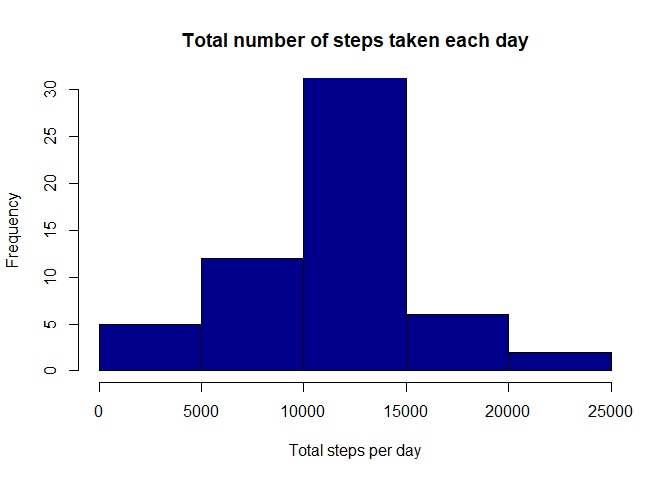
\includegraphics{reprodResearchProject1_files/figure-latex/unnamed-chunk-12-1.pdf}

\begin{Shaded}
\begin{Highlighting}[]
\NormalTok{mean\_steps\_day\_NA }\OtherTok{\textless{}{-}} \FunctionTok{mean}\NormalTok{(steps\_day\_NA}\SpecialCharTok{$}\NormalTok{steps)}
\NormalTok{median\_steps\_day\_NA }\OtherTok{\textless{}{-}} \FunctionTok{median}\NormalTok{(steps\_day\_NA}\SpecialCharTok{$}\NormalTok{steps)}
\end{Highlighting}
\end{Shaded}

La media no cambió después de los reemplazos de NA, la mediana cambió en
un porcentaje del 0,1\%.

¿Hay diferencias en los patrones de actividad entre los días de semana y
los fines de semana?

\begin{Shaded}
\begin{Highlighting}[]
\NormalTok{activity\_data\_NA}\SpecialCharTok{$}\NormalTok{date }\OtherTok{\textless{}{-}} \FunctionTok{as.Date}\NormalTok{(}\FunctionTok{strptime}\NormalTok{(activity\_data\_NA}\SpecialCharTok{$}\NormalTok{date, }\AttributeTok{format=}\StringTok{"\%Y{-}\%m{-}\%d"}\NormalTok{))}
\NormalTok{activity\_data\_NA}\SpecialCharTok{$}\NormalTok{day }\OtherTok{\textless{}{-}} \FunctionTok{weekdays}\NormalTok{(activity\_data\_NA}\SpecialCharTok{$}\NormalTok{date)}
\ControlFlowTok{for}\NormalTok{ (i }\ControlFlowTok{in} \DecValTok{1}\SpecialCharTok{:}\FunctionTok{nrow}\NormalTok{(activity\_data\_NA)) \{}
    \ControlFlowTok{if}\NormalTok{ (activity\_data\_NA[i,]}\SpecialCharTok{$}\NormalTok{day }\SpecialCharTok{\%in\%} \FunctionTok{c}\NormalTok{(}\StringTok{"Saturday"}\NormalTok{,}\StringTok{"Sunday"}\NormalTok{)) \{}
\NormalTok{        activity\_data\_NA[i,]}\SpecialCharTok{$}\NormalTok{day}\OtherTok{\textless{}{-}}\StringTok{"weekend"}
\NormalTok{    \}}
    \ControlFlowTok{else}\NormalTok{\{}
\NormalTok{        activity\_data\_NA[i,]}\SpecialCharTok{$}\NormalTok{day}\OtherTok{\textless{}{-}}\StringTok{"weekday"}
\NormalTok{    \}}
\NormalTok{\}}
\NormalTok{steps\_day }\OtherTok{\textless{}{-}} \FunctionTok{aggregate}\NormalTok{(activity\_data\_NA}\SpecialCharTok{$}\NormalTok{steps }\SpecialCharTok{\textasciitilde{}}\NormalTok{ activity\_data\_NA}\SpecialCharTok{$}\NormalTok{interval }\SpecialCharTok{+}\NormalTok{ activity\_data\_NA}\SpecialCharTok{$}\NormalTok{day, activity\_data\_NA, mean)}
\end{Highlighting}
\end{Shaded}

Gráfico de series de tiempo del intervalo de 5 minutos

\begin{Shaded}
\begin{Highlighting}[]
\FunctionTok{names}\NormalTok{(steps\_day) }\OtherTok{\textless{}{-}} \FunctionTok{c}\NormalTok{(}\StringTok{"interval"}\NormalTok{, }\StringTok{"day"}\NormalTok{, }\StringTok{"steps"}\NormalTok{)}
\FunctionTok{library}\NormalTok{(lattice)}
\FunctionTok{xyplot}\NormalTok{(steps }\SpecialCharTok{\textasciitilde{}}\NormalTok{ interval }\SpecialCharTok{|}\NormalTok{ day, steps\_day, }\AttributeTok{type =} \StringTok{"l"}\NormalTok{, }\AttributeTok{layout =} \FunctionTok{c}\NormalTok{(}\DecValTok{1}\NormalTok{, }\DecValTok{2}\NormalTok{), }
    \AttributeTok{xlab =} \StringTok{"Interval"}\NormalTok{, }\AttributeTok{ylab =} \StringTok{"Number of steps"}\NormalTok{)}
\end{Highlighting}
\end{Shaded}

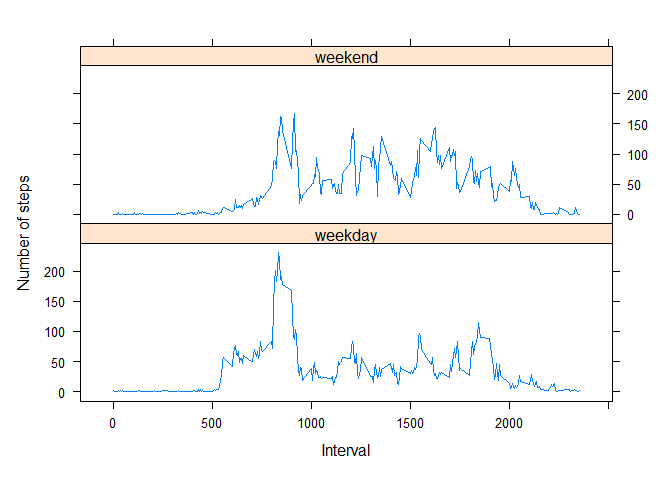
\includegraphics{reprodResearchProject1_files/figure-latex/unnamed-chunk-14-1.pdf}

\end{document}
